% Chapter Template

\chapter{Background} % Main chapter title

\label{Chapter2} % Change X to a consecutive number; for referencing this
% chapter elsewhere, use \ref{ChapterX}

\lhead{Chapter 2. \emph{Background}} % Change X to a consecutive number; this is
% for the header on each page - perhaps a shortened title

\section{Model Driven Engineering}
	
When a new software is created it has always been a goal to produce high
quality code at the lowest possible cost. To plan a software development project
from its initial start to delivering a finished product can seem like an impossible
thing to do. Because a software development cycle rarely goes as initially
planned. Changes do occur, both in delivering high quality code and keeping the
costs down. Traditionally when model driven engineering (MDE) is used, people
think about models, for example activity diagrams and class diagrams from the
popular modeling language, UML. Where models are used to raise the level
of abstraction for a problem specification and describes how the software
application should be implemented. For these software development processes
models are indirectly used in the creation of software. This means that models
are primarily used as a reference when implementing an application.

A model is an abstraction of a system, and has its origin from Latin,
\textit{modulus} that means measure or standard. A model can either be used to
represent a system before it is created or to describe some major aspects of a
system or a concept. When we hear the term model, many will think that it
is a miniature that consists of a set of nodes and arrows. But it is important
to consider that a model can also be represented by text. 

Considering traditional software development processes, models are
primarily used in application requirements and use-case diagrams to specify what 
the costumer wants. Developers can then specify models to detect important
functionality of the application. A software developer may for example create
flow charts, sequence diagrams, activity diagrams, class diagrams, etc, to
describe how the system should behave and be implemented. A model for system
architecture can also be initialized for developers to handle design choices. Rational
Unified Process\cite{Rational1998} (RUP) is an example of a software
development process that is build around extensive use of models in their
initial planning phase. RUP was initially created by Rational Software
Corporation\cite{IBMRational} in 2006 and was later acquired by International
Business Machines Corporation\cite{IBM}. This is an iterative software
development process and the purpose of RUP is to be an adaptable process
framework where the software project teams decide the elements that are
required for a development cycle. Figure~\ref{fig:RUP} explains the four
different phases, Inception, Elaboration, Construction and Transition, with
different iterations for each phase that RUP provides. The Inception phase and
the Elaboration phase is the two phases where some of the example models above
are created, both under business modeling and requirements. For the Inception
phase the idea is to create the software application without writing
any source code. This phase is  concerned with writing text and creating models
that gives the developers a detailed specification on how the program should be
implemented. In the Elaboration phase a prototype might be implemented to show
the customer a possible implementation, but this phase also consist of creating
and modifying an extensive amount text and models that specifies analysis and
design choices. The goal for these two phases is to define a solid foundation of
the application before starting to write code and tests.
In the Construction phase the developers should know exactly how the application
should be implemented by referring to documents and models created in earlier
phases. RUP is only one example of how a software development process could be
applied to a project. Agile development processes has become popular the last
couple of years, where processes like Scrum\cite{Schwaber2001} and Extreme
Programming\cite{Beck1999} (XP) has been integrated in software development
teams all over the world. Both Scrum and XP thrives to focus more on the
implementation and on delivering high quality code than on creating documents
and models. However, models will always be a tool for developers, also in agile
development processes, when some aspects of a system needs to be explained.
Because to explain parts of an implementation with a model will help to make
the explanation less complex and more abstract.

\begin{figure}[H]
	\centering
	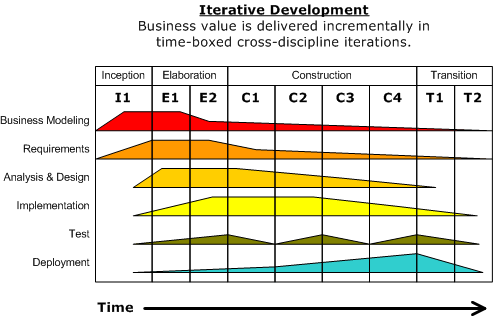
\includegraphics[scale=0.7]{./Figures/RUP.png}
	\caption[Rational Unified Process]
	{Iterative development cycle of Rational Unified Process.}
	\label{fig:RUP}
\end{figure}

Now we have acknowledged some development processes that are commonly used in
the industry for creating software applications. Model Driven Engineering is a
software development methodology that focus on creating and exploiting
models. And by using these models, MDE aims at improving productivity and
quality in a software developments\cite{France2007}. This is achieved by not only to use
models as documentation, but instead use models as the major artifact in a software
development cycle. The idea is to use models at different levels of abstraction
and apply model transformations to automate the implementation of these
models. This will raise the level of abstraction in program and problem
specification. We can divide these models into two main model classes, namely
development models and runtime models. Development models are used as an
abstraction above code level. These models can represent software
requirements, work flow, architecture and software implementation. These
development models are most commonly used in software development processes as a
supplement in developing an application. Runtime models represents executable
systems of a software application. Example of such executable systems are
database operations or computations of data. There has been an increase in MDE
researchers that explore how runtime models can be used to support dynamic
adaptation of systems for a software application\cite{France2007}. The idea for
MDE is to be able to specify these development models as runtime models and
evolve software applications with the use of runtime models and development
models as major artifacts of a development process. 
 
A typical Model Driven Software Engineering (MDSE) scenario is to obtain an
executable software application through model transformations that produce a
more and more detailed version of the application until an executable version is
created. We reach this level of automation by applying model transformations to
models at higher levels of abstraction and producing models that contains a more
detailed description of the software. This highlights one main advantage of a
model driven approach, and that is to bridge the communication gap between
requirements/analysis and implementation\cite{Brown2008}. For a traditional
development process today there is a gap in communication between software
developers and customers\cite{France2007}. Because a customer is usually not an
expert in designing and implementing a software application. A customer can
provide a set of requirements for a software application and take part in
analysing these requirements to make sure that the development team shares the
customers thought of the program. The requirements and analysis can be
specified down to every detail, however a software application might experience
different design choices that leads to a different implementation of the
application compared to what the costumer initially specified. If the visions
of MDE is adopted to a software development process then this could help to
narrow the gap in communication between developers and stakeholders. Because
now we can apply model transformation that changes input models to target
models that represents both the design and the executable implementation of a
software application. We will describe model transformations and their purpose
in model driven engineering in more depths in chapter~\ref{Chapter3}. Models
that are provided at different level of abstractions is less complex than
several thousand lines of implementation code. This represents another benefit
of adopting MDSE into the development process. Because models captures and
organize the understanding of a system that results in a more clear discussions
among team members and new team members. One approach that introduces modeling
at different level of abstraction for including MDSE in a software development
process is the Model Driven Architecture.

\subsection{Model Driven Architecture}
\label{MDA}

Model Driven Architecture (MDA) is an industry architecture developed by the
Object Management Group (OMG) that address the possibility to provide automation
according to models in an application development cycle.
MDA is a proposal for applying the practices of MDE to a system development. This
architecture is a good example to use when we are discussing concepts of MDE,
because of its similarity to a traditional software development process. Since
it has support for standard phases in a software development process such as
analysis, design and implementation. Many organizations have adopted MDA as a
reference framework to include the concepts of MDE. One reason for this is the
importance of OMG for the software industry. MDA is build around many
concepts that OMG has released, such as the OMG specifications the Unified
Modeling Language (UML) and the Meta Object Facility(MOF).

\begin{figure}[H]
	\centering
	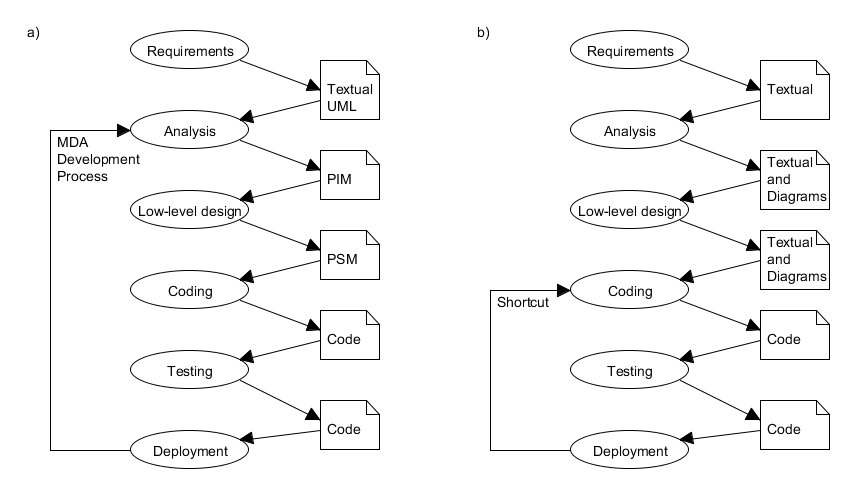
\includegraphics[scale=0.5]{./Figures/MDA.png}
	\caption[Software Development with MDA]
	{a) Model-Driven-Architecture and b) Traditional development process}
	\label{fig:MDA}
\end{figure}

Figure~\ref{fig:MDA} gives a representation of the development process that the
Model Driven Architecture provides and a traditional development process on the
right side.
Both of the approaches have similar starting phases, where a customer presents a
list of requirements for a software application. The process to create
implementation code from the requirements is where a MDE approach to software
development is different. Because for MDA the idea is to use models instead of
text and diagrams for the analysis and design phase. For a traditional
development process these phases usually consist of creating diagrams that
describes different system of the application. In MDA these diagrams or models
are the main artifact for the corresponding phases, instead of just a reference for
developers to use when implementing an application. The architecture then
propose that implementation code is generated based on these models. A
traditional software development process would have iterations for the
implementation and testing to make sure that the application meets the demands
of the customer. This process is continued for every iteration, where
developers continually use the text and diagrams that was created earlier in
the process. The idea for an MDA development process is to provide automation
between models created at each development phase. Instead of going back to the
code and do corrections and modifications on the application a model driven
software development process goes back to analysing the problem and modify the
models accordingly. With the power of automatically changing models from one
phase to another and generate implementation code from the models at the last
level of abstraction.

Figure~\ref{fig:MDA_PLATFORM} provides a representation of the models at the
different layer of abstractions that is part of the Model Driven Architecture. 

\textbf{Computation-Independent Model (CIM)} is the most abstract level of
modeling and is often referred to as a business model or domain model. The
model does not contain any computational implications to how the software
application should behave, but express exactly what the final application
should do. This model remains independent to how a system will be or currently
is implemented and represents the requirements and purpose of the system. A
Computation-Independent Model is often described by using a natural language to
define the requirements for a software application. 

\begin{figure}[H]
	\centering
	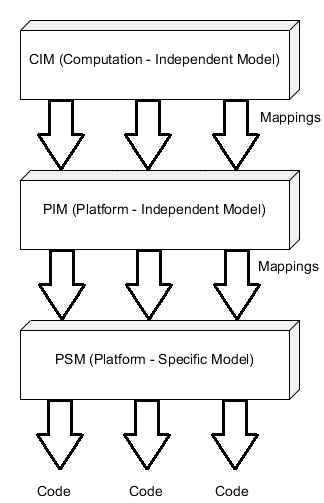
\includegraphics[scale=0.7]{./Figures/MDA_Platforms.png}
	\caption[The three levels of modeling abstraction for MDA]
	{The three levels of modeling abstraction that MDA provides.}
	\label{fig:MDA_PLATFORM}
\end{figure}

\textbf{Platform-Independent Model (PIM)} is the level of abstraction that
describes the behavior and structure of a software application. This model is
platform independent, which means that the technological platform used to
implement the software application is not defined. A Platform-Independent Model
will only address tasks that a software application can perform. These tasks
are part of the context of the business model at the top level of abstraction.

\textbf{Platform-Specific Model (PSM)} is the level of abstraction that contains
all required information for the behavior and structure of a software
application that is linked to a specific technological platform. These specific
platform technologies can be a specific programming language like a general
purpose programming language, a specific operation system or a specific database
technology. The Platform-Specific Model contains all the information that is
required for an actual implementation of the application. 

In MDA, the core activity is the starting phase, which is to analyse the
problem at hand. Requirements are firstly defined and modeled as a CIM or a PIM.
The CIM and PIM provides the solution for the requirements at a very high level
of abstraction. The computation independent level of abstraction we provide
the requirements of a solution without thinking about the actual implementation
of an application. A CIM specifies the workflow of an application and how end
users utilizes the application. For example the model could define the
requirements for a web application that provides a collection of goods that the end users can purchase.
These requirements could specify how an employee performs tasks when a new order
arrives. For the implementation of an application not all of these requirements
are necessary. The purpose of MDA is that models created at
CIM level provides the highest level of abstraction and therefore should be
readable by everyone. In figure~\ref{fig:MDA_PLATFORM} MDA suggest
that new models are created accordingly based on a set of mappings. Models that
is provided at the platform independent abstraction is not concerned with
technologies that should be used for the actual implementation. PSM is more
concerned with describing what tasks an application should perform. But tasks
that an employee should perform, like for example making a shipment ready for
transportation is not defined in a PIM. A platform specific model specifies what
implementation platform and a set of precise descriptions of the technical
details of the corresponding implementation platform. Mapping a model to another
model is essential for applying MDA to a development process. A mapping defines
correspondences between elements of two different models and can be defined
between all different models.

\section{Modeling Languages}

A Modeling language is defined through three core concepts. Regardless if its
either a Domain Specific Modeling Language (DSML) or a General Purpose Modeling
Language (GPML). Figure~\ref{fig:modeling_language} represents the three main
concepts for a modeling language.

\begin{figure}[H]
	\centering
	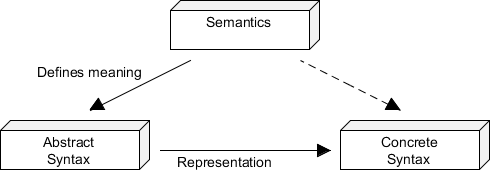
\includegraphics[scale=0.7]{./Figures/modeling_language.png}
	\caption[Main ingredients of a modeling lanugage.]
	{The three main ingredients of a modeling language.}
	\label{fig:modeling_language}
\end{figure}

A modeling language has an abstract and a concrete syntax. The abstract syntax
describes the structure of the modeling language and how modeling elements can
be combined together. The concrete syntax on the other hand describes a specific
representation of the abstract syntax, and can either be a graphical or
textual representation. The semantics of a modeling language describes the
meaning of these modeling elements and the different ways to combine them for
the abstract syntax and indirectly the concrete syntax. We mentioned DSML and
GPML, where these two modeling languages represents one of the main
classification of modeling languages. A modeling language can either be
classified as a domain specific or a general purpose language. DSMLs are
modeling languages that are designed for a specific domain or a concept. While
GPMLs are modeling languages that is applicable for several different domains.
A general purpose language lacks features that are special for a particular
domain. This is one of the strengths for DSLs that is created especially for a
certain domain, and therefore provide more details to a specific domain compared
to a general purpose language. The Unified Modeling Language\cite{UML_SPEC}
(UML) is an example of a general-purpose modeling language that
was accepted in 2000 by the International Organization for Standardization
(ISO) as an industry standard for modeling software systems. UML was initially
developed by Grady Booch, Ivar Jacobsen and James Rumbaugh at Rational Software
in the 1990s. It was later adopted by the Object Management Group in 1997 and
has since this day been continuously developed by the organisation. UML is
often called a general purpose language because it is often referred to as a
suite of languages, since it provides developers and designers with the possibility to
specify applications through several different modeling languages, or diagram
types that UML often is associated with. However, in the book, ``Model-Driven
Software Engineering in Practice'' published by Marco
Brambilla, Jordi Cabot and Manuel Wimmer in 2012, they state the following.
\textit{If we think to the general modeling problem, we can see UML as
a DSL tailored to the specification of (mainly object-oriented) software
systems\cite{Brambilla:MDSE}.} This means that to decide whether UML is a DSL or
a GPL is not a binary choice. But we mostly see UML as a general purpose
modeling language, since it offers a wide variety of modeling languages that
designers and developers can use to specify system abstractions. Whether a
modeling language is classified as a general purpose or a domain specific
modeling language it requires that it is described by an abstract syntax. Both
the abstract syntax and the concrete syntax of a modeling language is
represented as models. Therefore the specification of the abstract syntax is
often referred to as a meta-model. 

\subsection{Meta-modeling}

Models are a major artifact in the concept of model driven engineering (MDE). It
is essential to look at every model as instances of some more abstract model.
And therefore we can define a meta-model as yet another abstraction that
highlights the properties of an instance model. Meta-modeling represents a vital
part of MDE and constitutes the definition of a modeling language. A meta-model
defines the abstract syntax and provides a description of a modeling language.
Another popular definition for describing a meta-modeling is that it is a
``model of models". This definition is both unhelpful and incorrect according
to Steve Cook and Stuart Kent in their paper\cite{Cook2008} published in 2008.
They think that a better definition for a meta-model is that ``it is a model of
the concepts expressed by a modeling language.'' The exact definition of a
meta-model is highly debated amongst MDE researchers\cite{Rutle_thesis}.

\begin{figure}[H]
	\centering
	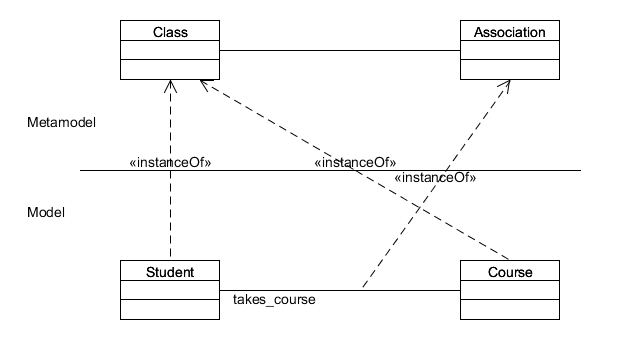
\includegraphics[scale=0.6]{./Figures/SimpleMetamodel.png}
	\caption[Example of a model and meta-model]
	{A simple example of a model and its meta-model.}
	\label{fig:SimpleMeta-model}
\end{figure}

Figure~\ref{fig:SimpleMeta-model} shows a simple example of an instance model
and its corresponding meta-model. This model has two classes, Student and Course, and
a bidirectional association, take course and has students, that relate
these two classes. The model is specified by a meta-model that consists of two
meta-classes Class and Association and an association between them. Both Student
and Course are an instance of the meta-class Class, while the association
between Student and Course are instance of the meta-class Association. The
modeling language that describes this model corresponds to the Unified Modelling
Language.

\subsubsection*{Meta-Object Facility}

The Meta-Object Facility\cite{MOF} (MOF) is an Object Management Group standard
for defining meta-models in MDE. The Object Management Group was in need of a
architecture to define the UML. Through this process of finding a common
platform for UML, OMG designed a four layered architecture that provides a
semi-formal approach to creating meta-models. MOF later became a language for
defining abstract syntax for modeling languages. 

\begin{figure}[H]
	\centering
	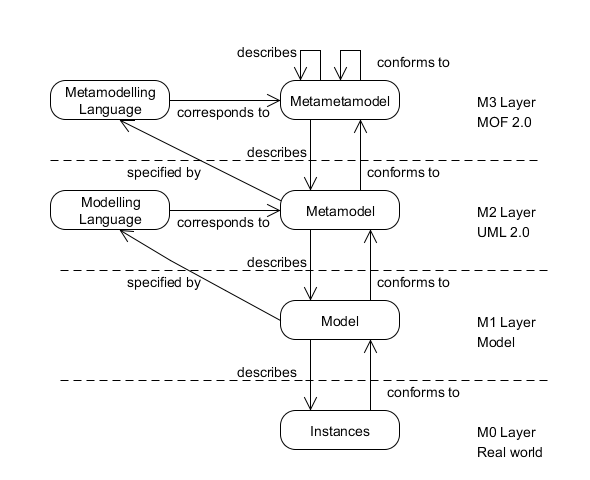
\includegraphics[scale=0.6]{./Figures/MOFLayers.png}
	\caption[Meta Object Facility]
	{Example of Meta Object Facility and its four layers.}
	\label{fig:MOFLayers}
\end{figure}

Figure~\ref{fig:MOFLayers} gives a impression of the four layers that are
available in the Meta-Object Facility. At the top level, M\textsubscript{3},
there is a meta-meta-model called MOF. This meta-meta-model is meant to both
describe it self and conform to itself. MOF is then used to describe meta-models
at the M\textsubscript{2} level. The UML meta-model is an example of such a
meta-model. The idea is that these meta-models are specified by some
meta-modeling language that corresponds to MOF. Models at the M\textsubscript{2}
layer represents the abstract syntax for models created in the M\textsubscript{1} layer. This
layer represents models that are created by some modeling language, like
for example UML. Finally at the M\textsubscript{0} we have an instance model of
a real world object. If we refer to our simple example concerning a model and
its corresponding meta-model in figure~\ref{fig:SimpleMeta-model}. From this
example we can create a real world object of that model, ``Petter Barvik'' takes
a course in Model Transformations. MOF provides meta-modeling architecture where
every modeling element on every layer corresponds to some modeling element
one layer higher. One could say that MOF itself a Domain Specific Language (DSL)
to create meta-models. 
 
\subsection{Constraints}

Constraints impose conditions that modeling elements must satisfy and helps
to define the semantics of a domain specific language. A constraints can be
compared to a Boolean condition. Boolean conditions are either true or false,
while constraints are either satisfied or not satisfied. Including constraints
to modeling elements in the abstract syntax specifies how modeling elements
are presented in an instance model. Modeling elements that are included in the
abstract syntax can have constraints defined on objects, classes, attributes, links,
associations, etc. A constraint is a restriction for how these elements should
behave. Constraints on elements such as those above can be expressed with a
natural language or by a formal language, such as the Object Constraint
Language\cite{OCL} (OCL). The Object Constraint Language (OCL) is a declarative
programming language for describing constraints that applies to UML models.
Before UML became an adopted standard of the Object Management Group (OMG), OCL
was an extension language to UML. Now OCL can be used with any Meta-Object
Facility (MOF) meta-model, including UML. A software developer can in
combination with UML and OCL define the semantics for a modeling
language\cite{Warmer:2003:OCL:861416}.

The difference between object and classes needs to be specified. A class
is often a meta element for an object. This means that a class could be part of
a model that describes an object element, and therefore an object element is
typed by the class element\cite{OO_UML}. Figure~\ref{fig:SimpleMeta-model}
describes the two object elements Student and Course that are an instance of the
meta-element Class.

\begin{figure}[H]
	\centering
	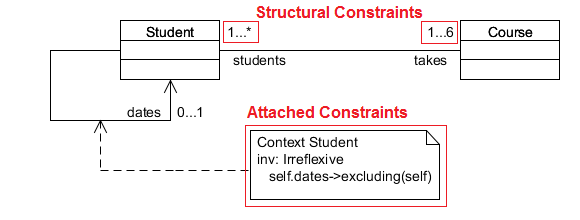
\includegraphics[scale=0.7]{./Figures/Constraints.png}
	\caption[Simple model with constraints]
	{Example of a simple model with attached and structural constraints.}
	\label{fig:Constraints}
\end{figure}

These restrictions on modeling elements can either be a structural constraint or
an attached constraint. These structural constraints are defined in the structure
of the models. In figure~\ref{fig:Constraints} we have extended the model we
introduced in figure~\ref{fig:SimpleMeta-model} with some  modeling elements. We
have created an association that specifies that a student can date other
students. In this model we can see that the model has three multiplicity
constraints that are part of the models structure. A multiplicity constraint for
an association restricts the number of objects that are related to a given
object. From the association constraint on this model we can see that a student
requires to take at least one course and up to a maximum of six courses. The
models restricts a student to not participate in any courses. The second
structural constraint requires a course to have at least one student for
this course to be part of a semester, and the course can have an arbitrary
maximum number of students participating the course. The association dates,
between two students for this model has an attached constraint that is
specified in the declarative language OCL. The general form of an attached
constraint has a context, in this case a Student, that specifies what object the
constraint includes. The attached constraint has a name \textit{``Irreflexive''}
followed by a Boolean OCL expression that explicitly refers to itself. This constraint
specifies that a student is unable to date her or him self. Constraints has a
vital part in model driven engineering to measure the quality and precision of a
model. A model without constraints does not work in practice. In
\textit{The Object Constraint Language: Getting Your Models Ready for
MDA}\cite{Warmer:2003:OCL:861416}, Jos Warmer and Anneke Kleppe states that a
model without constraints would be severely underspecified. Constraints
expressions written in OCL are unambiguous and results in a more precise and
detailed model. If we where to remove both the structural and attached
constraints from figure~\ref{fig:Constraints} then the model is less
informative. There is no understanding on how the objects are related to
one another. 

\section{Language Workbenches}

Language workbenches are tools that lets user specify
their own Domain Specific Language (DSL) and include editing tools for the newly
created language. A workbench should consist of Integrated Development
Environment (IDE) that lets users create their own DSMLs.
Figure~\ref{fig:langauge_workbench} is provided in the paper, \textit{``DPF
Workbench: a multi-level language workbench for MDE"}, that was published by
Yngve Lamo, Xiaoliang Wang, Florian Mantz, {\O}yvind Bech, Anders Sandven and
Adrian Rutle in 2013. The figure presents the intended use of language
workbenches and consist of two phases. The first handles the definition of a
new DSML and the creation of tool support such as code generation, editors,
model transformations, etc. A language workbench is created by a domain expert
in collaboration with an experienced developer. The latter describes the actual
usage of this newly created workbench, where developers can utilize the DSML
environment to create models, generate implementation code, etc. Language
workbenches are a very young field in computer science, and there are many
existing solutions that is open for the public to use. These concepts have the
potential to change the face of programming as we know
it\cite{fowler2010domain}, but the concepts of workbenches are still fresh to
computer science.

\begin{figure}[H]
	\centering
	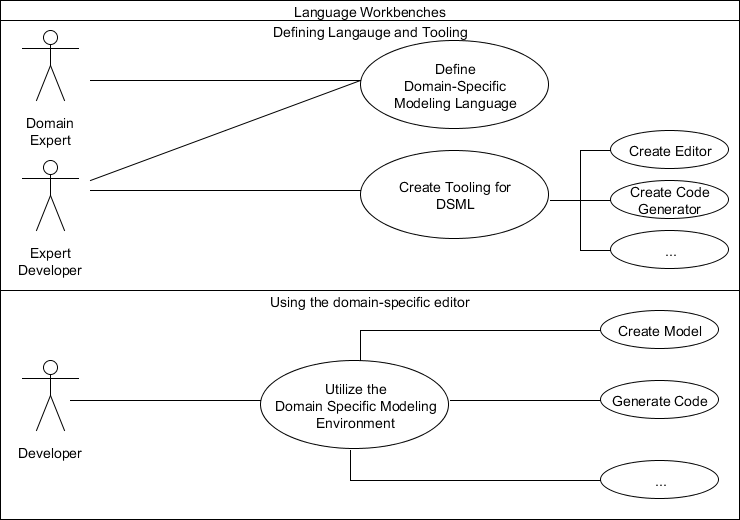
\includegraphics[scale=0.6]{./Figures/langauge_workbehcn.png}
	\caption[Intended use of language workbenches]
	{Intended use of language workbenches.}
	\label{fig:langauge_workbench}
\end{figure}

The concepts behind a language workbench is that the tool does not just provide
the users with an IDE to create DSLs, but also generates a new IDE where this
newly created DSL can be edited. In addition to an IDE that provides creation
and editing of a newly created language a workbench should define support for
code generation, model transformation, model versioning, etc\cite{Lamo2013}.
Figure~\ref{fig:workbench} describes components for a language workbench. Martin
Fowler describes three main parts to defining a new language workbench in his
paper\cite{fowler2005language}:

\begin{figure}[H]
	\centering
	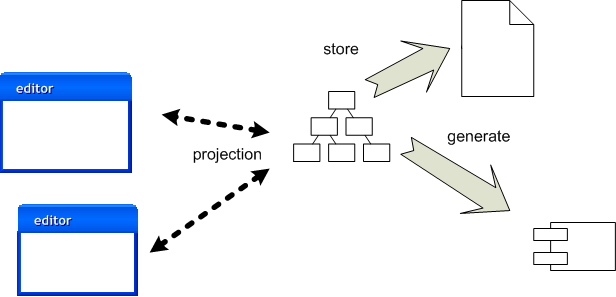
\includegraphics[scale=0.6]{./Figures/workbench.png}
	\caption[Components of language workbenches]
	{Components of language workbenches.}
	\label{fig:workbench}
\end{figure}

\begin{itemize}
  \item The abstract representation for the language.
  \item One or more editing environments for the language.
  \item Defining the semantics behavior of the language. 
\end{itemize}

\subsection{EMF}

Eclipse Modeling Framework is originally based on Meta Object Facility (MOF)
provided by the Object Management Group (OMG). In 2003 EMF designers contributed
to designing the MOF 2.0 version of the standard that was later named Essential
MOF (EMOF). EMF provides the meta-model Ecore that is aligned to EMOF and is a
general purpose modeling language to create modeling languages. Ecore is
essentially a simplified version of class modeling in UML.

\begin{figure}[H]
	\centering
	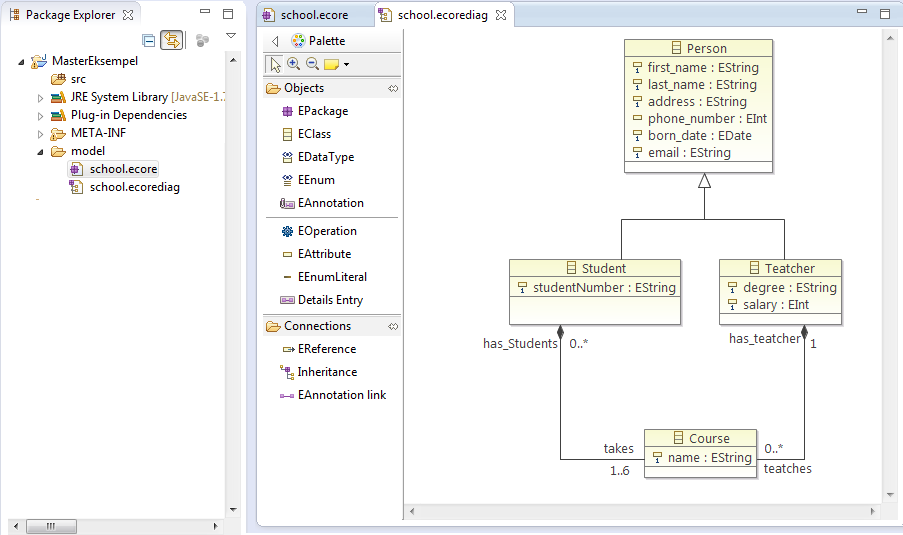
\includegraphics[scale=0.6]{./Figures/EMF_Diagram_Picture.png}
	\caption[Ecore model represented by Ecore Tools]
	{A graphical representation of an Ecore model.}
	\label{fig:EMF_Diagram}
\end{figure}

Figure~\ref{fig:EMF_Diagram} represents an Ecore model that is created from a
graphical editor. This Ecore model conforms to the Ecore meta-model and is the
core language for EMF. The framework provides a two layered approach to
meta-modeling where the user can create a DSL based on the Ecore meta-model.
Based on the DSL the framework provides code generation facilities. Amongst
generating java implementation for the model the framework also provides code
generation for an editor that is based on the DSL. This editor can be used to
create instances of the defined DSL. 

% \subsection{Visual Modeling and Transformation System}

% \begin{figure}[H]
% 	\centering
% 	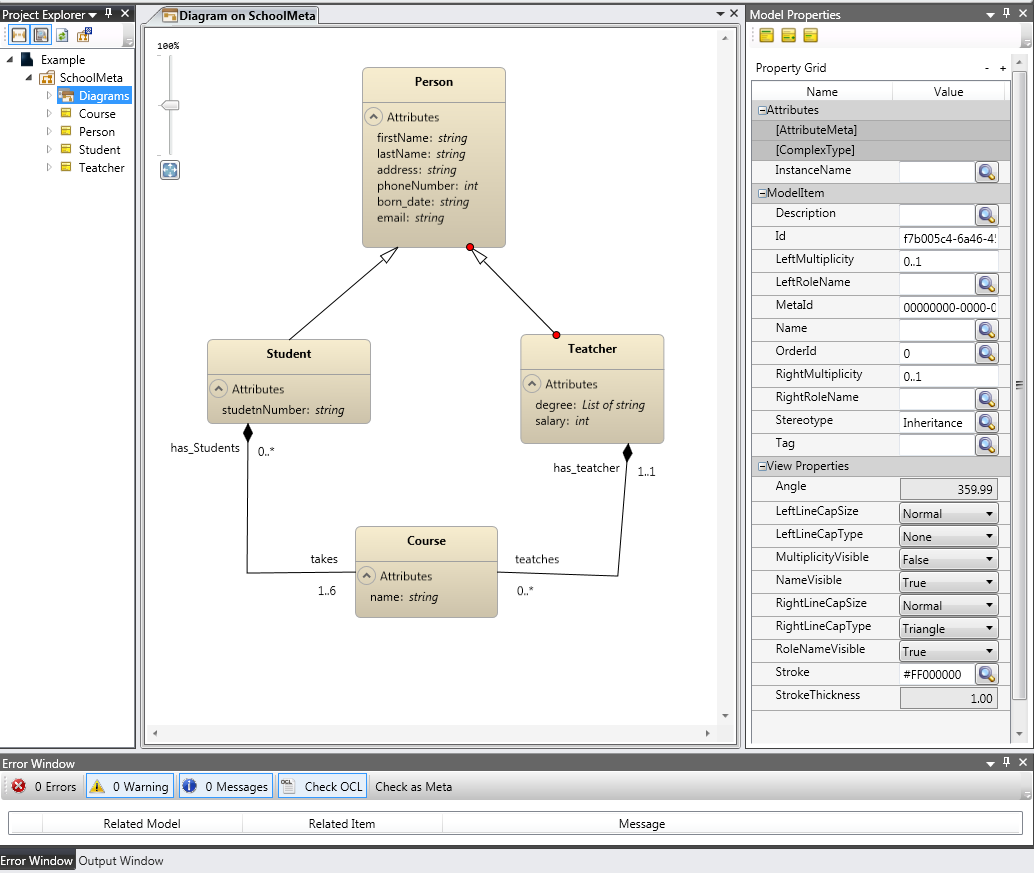
\includegraphics[scale=0.5]{./Figures/VMTS}
% 	\caption[Creating domain specific modeling language in VMTS]
% % 	{Specifying a domain specific modeling language in VMTS.}
% 	\label{fig:VMTS}
% \end{figure}

\section{Diagram Predicate Framework}
\label{sec:DPF}

Diagram Predicate Framework\cite{Rutle_thesis,Rossini_thesis,Lamo2013} (DPF) is
an ongoing research project that was first initiated by Bergen University
Collage and the University of Bergen in Norway 2006. With features likes
meta-modeling, model transformation and model management, DPF aims at
formalising concepts of model-driven engineering. DPF is based on category
theory and graph transformations and is an extension of the Generalised
Sketches\cite{Diskin2003} formalism that was initially developed by Zinovy
Diskin.

In October 2002 Dominique Duval published a paper where he specified that a
specification can be considered as a directed graph with additional structure
in the same way that a theory can be considered as a category with additional
structures\cite{Duval2003}. Generalised Sketches by Zinovy Diskin utilize the
concept of sketches. A sketch, first introduced by Ehresman in 1966, is a
directed graph that provides additional properties, such as colimit, limit and
constraints. DPF utilize these concepts through an diagrammatic approach to
meta-modeling and to facilitate the concepts of MDE. The framework provides the
possibility to define an unlimited layers of meta-modeling. In DPF models are
represented as specifications.

\begin{itemize}
  
\item A \emph{specification $\spec{S}$} = (S,
C\textsuperscript{$\spec{S}$}:$\Sigma$) consist of an underlying graph S and a
set of atomic constraints C\textsuperscript{$\spec{S}$}. 

\item Atomic constraints are specified by predicates from a predefined signature
$\Sigma$.

\item A signature $\Sigma$ = ($\Pi$ \hspace{1 mm}, \hspace{1 mm}$\alpha$)
consist of a collection of predicates. 
  
\end{itemize}

A \emph{specification $\spec{S}$} has an underlying graph S that contains
modeling elements that defines the model structure of the specification. These
modeling elements are always represented as a node or an arrow. However these
nodes and arrows could be specified through several layers of
meta-models or specifications. The \emph{specification $\spec{S}$} also consist
of a set of constraints, these constraints will restrict the model structure of
a new instance model of this specification. Figure~\ref{fig:DPF_Spec} presents a
specification $\spec{S}$\textsubscript{2}, that is defined by an underlying
specification $\spec{S}$\textsubscript{3} and describes a modeling language for
some $\spec{S}$\textsubscript{1} specification. This specification includes two
nodes Condition and Activity, two arrows ChoiceOut and Message and  two sets of
atomic constraints. The first constraint defines that a Condition element has
to be connected to exactly one Activity element for this structure. The second
constraints specifies for this graph structure that an Activity element cannot
be associated with it self. These constraints examples are specified as a
collection of predicates from a predefined signature $\Sigma$. The table in
figure~\ref{fig:DPF_Spec} represent some of the predicates from this
collection. A predicate is represented by an unique symbol $\Pi$, a shape graph
$\alpha$, a proposed visualisation and a semantic interpretation

\begin{figure}[H]
	\centering
	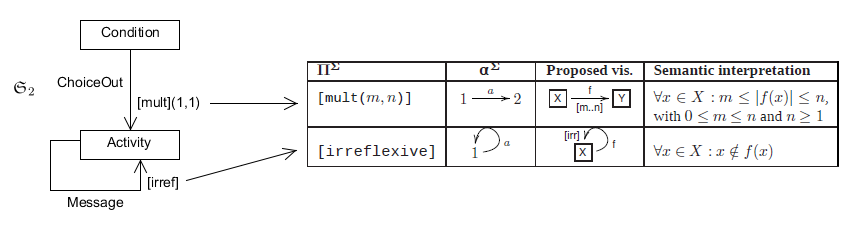
\includegraphics[scale=0.7]{./Figures/DPF_spec_constraints.png}
	\caption[A specification and some predefined diagrammatic predicate attached]
	{A specification $\spec{S}$\textsubscript{2} with some attached predicates.}
	\label{fig:DPF_Spec}
\end{figure}

An instance specification $\spec{S}$\textsubscript{n} that is initialised from
a specification $\spec{S}$\textsubscript{n+1} defines a graph homomorphism
between two underlying graphs. There is a graph homomorphism,
S\textsubscript{n}$\longrightarrow$S\textsubscript{n+1}, between the underlying
graph S\textsubscript{n} of a specification $\spec{S}$\textsubscript{n} and the
underlying graph S\textsubscript{n+1} of
a specification $\spec{S}$\textsubscript{n+1}\cite{Lamo2013}. The graph
homomorphism S\textsubscript{n}$\longrightarrow$S\textsubscript{n+1} must
satisfy a set of atomic constraints, C\textsuperscript{$\spec{S}$} from a
specification $\spec{S}$\textsubscript{n+1}.
Figure~\ref{fig:modeling_formlalism} from Adrian Rutle's dissertation,
 \textit{Diagram Predicate Framework A Formal Approach to
MDE}\cite{Rutle_thesis} that was published in 2010 represents an example of a
specification that is defined by a modeling formalism. 

\begin{figure}[H]
	\centering
	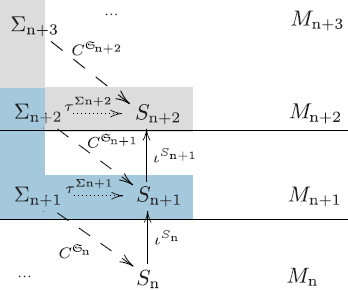
\includegraphics[scale=0.7]{./Figures/modeling_formlalism_adrian.png}
	\caption[Modeling formalism in DPF]
	{Meta-modeling represented as modeling formalism's in DPF.}
	\label{fig:modeling_formlalism}
\end{figure}

Because in DPF a modeling language at a specific abstraction layer is
represented as a modeling formalism.
A modeling formalism in DPF is defined by a set of atomic constraints from a
modeling formalism one abstraction layer higher and a specification that has an
underlying graph and a set of atomic constraints. For example figure~\ref{fig:modeling_formlalism} represents three levels of
abstractions for defining a DSML. The specification $\spec{S}$\textsubscript{n}
that is defined at M\textsubscript{n} layer conforms to the modeling
formalism one layer higher. The modeling formalism consist of a specification
$\spec{S}$\textsubscript{n+1} that has an underlying graph S\textsubscript{n+1}
and a set of predicates Z\textsubscript{n+2}. Together with specification
$\spec{S}$\textsubscript{n+1} a set of predicates Z\textsubscript{n+1} can be
defined to specify a new modeling formalism for lower layer of abstractions. 
modeling formalism\cite{Rutle_thesis}. This defined modeling language, or
modeling formalism provides the abstract syntax that can be used to create a
specification or modeling formalism one abstraction layer lower. What is special
with DPF is that a modeling formalism represents both the abstract syntax for
a specification one abstraction layer lower and the concrete syntax for a
specification one abstraction layer higher. The set of atomic constraints
Z\textsubscript{n+1} provides the semantics and the
specification $\spec{S}$\textsubscript{n+1} provides the abstract syntax for
defining modeling elements in a new specification $\spec{S}$\textsubscript{n}.
Figure~\ref{fig:MOF_vs_DPF} explains the difference between OMG's MOF and DPF's
multi-layered meta-modeling hierarchy.

\begin{figure}[H]
	\centering
	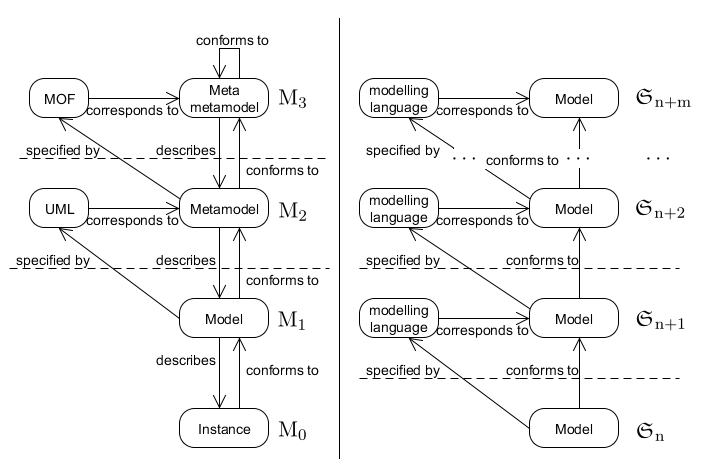
\includegraphics[scale=0.7]{./Figures/MOF_vs_DPF}
	\caption[OMG's layers of meta-modeling and multilayer modeling]
	{OMG's layers of meta-modeling and an arbitrary layer of meta-modeling.}
	\label{fig:MOF_vs_DPF}
\end{figure}

These two sides highlights the differences between DPF and modeling environments
that expand MOF to create modeling languages. While MOF based modeling
environments provides two abstraction layers, DPF on the other hand provides an
unlimited abstraction layers users can interact with. The reason that MOF based
modeling environments provides two layers to interact with is because the
layers M\textsubscript{2} and M\textsubscript{3} are usually part of the
environments internal infrastructure. For example in EMF users can create
models that conforms to the Ecore meta-model. The only meta-model that users of
DPF are unable to interact with is located at the highest abstraction layer. A
specification $\spec{S}$\textsubscript{n+1} is specified by a modeling language
that corresponds to a specification $\spec{S}$\textsubscript{n+2}. But the same
specification $\spec{S}$\textsubscript{n+1} also represents the abstract syntax
for a specification $\spec{S}$\textsubscript{n}. These DPF models automatically
generates a new graphical editor environment provided by the DPF Workbench.

\section{DPF Workbench}

The DPF Workbench provides a modeling environment for DPF and consist of three
main components. These are the ``DPF Model Editor'', the ``DPF Signature Editor''
and the ``DPF Code Generator''. The first two editors provides the modeling
functionality for the DPF Workbench. ``DPF Model Editor'' is used to create and
modify DPF specifications. The ``DPF Signature Editor'' is used as a supplement
to the ``DPF Model Editor''. It provides an editor to construct user defined
predicate signatures. These signatures can then be used to define the semantics
of a DPF specification in the ``DPF Model Editor'' if the predefined predicates
that DPF provides does not suffice. Figure~\ref{fig:DPF_Editor} that is
provided in the article\cite{Lamo2013}, explains how the ``DPF Signature Editor'',
the ``DPF Model Editor'' and a DPF Model is related to each other in the DPF
Workbench over different abstraction layers. The ``DPF Code Generator'' provides
the users with a code generation environment for DPF specifications.  

\begin{figure}[H]
	\centering
	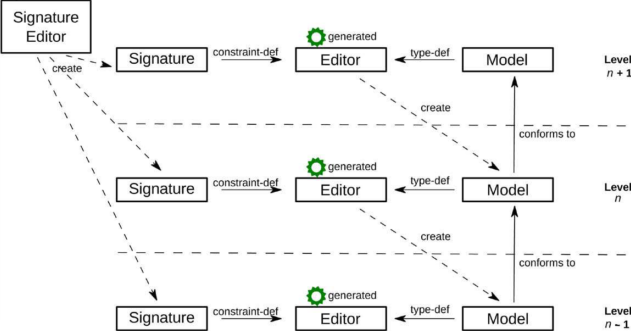
\includegraphics[scale=0.7]{./Figures/DPF_Workbench}
	\caption[DPF Editor in multi-layer meta-modeling hierarchy]
	{Generated DPF Editors in a multi-layer meta-modeling hierarchy.}
	\label{fig:DPF_Editor}
\end{figure}

\subsection*{DPF Model Editor}
The DPF Model Editor is an extension of the Diagram Predicate Framework that
provides an intuitive approach to creating modeling languages and have been created
using several different technologies. In 2011 $\O$yvind Bech published his
master thesis\cite{Bech_thesis} where he designed the implementation of
the DPF Model Editor that is based on the Eclipse Modeling Framework technology.
This first version of the DPF Model Editor has seen several iterations and provides
support for creating domain specific modeling languages.
Figure~\ref{fig:DPF_Editor} explains that a new instance of the DPF Model
Editor is generated for each new model that is created. This means that every
DPF specification has a corresponding editor that provides graphical editing
properties to change the models. For each generated editor we can create a new
DSL one abstraction layer lower that generates a new editor that correspond to
this DSL.

% \subsection*{DPF Signature Editor}
% 
% \subsection*{DPF Code Generator}

%  
% \begin{table}[ht]
% \renewcommand*\arraystretch{1.5}
% \centering
% \begin{tabular}{| c | c | c | c | c | c |}
% \hline
% Tool & Layers & Dia.   & Const.   & Platform & GUI\\
% 	 & 		  & Const. & Language &          & \\
% \hline
% EMF/GMF & 2 & & OCL, EVL, & Java VM & $\surd$ \\
% 		%&  	& & Java      &         & \\
% \hline
% VMTS    & $\infty$ & & OCL & Windows & $\surd$ \\
% \hline
% AToM\textsuperscript{3} & 2 & & OCL, Python & Python, Tk/tcl & $\surd$ \\
% \hline
% GME  & 2 & & OCL & Windows & $\surd$ \\
% \hline
% metaDepth & $\infty$ & & EVL & Java VM & \\
% \hline
% DPF & $\infty$ & $\surd$ & Predefined & Java VM & $\surd$ \\
% 	& 		   &         & validator  &         & \\
% \hline
% 
% \end{tabular}
% \caption{Comparing model transformation tools.}
% \end{table} 
